\documentclass[11pt]{article}
\usepackage[T1]{fontenc}
\renewcommand{\rmdefault}{ptm}
\usepackage[paperwidth=297mm,paperheight=210mm,margin=0mm]{geometry}
\usepackage{amsmath,amssymb,booktabs,graphicx,tikz}
\usetikzlibrary{arrows.meta,calc}
\definecolor{ink}{HTML}{243746}
\definecolor{axa}{HTML}{D17B14}
\definecolor{axd}{HTML}{963D98}
\definecolor{axx}{HTML}{1765B0}
\definecolor{axy}{HTML}{C43C39}
\definecolor{axz}{HTML}{22854E}
\pagestyle{empty}
\begin{document}\null
\begin{tikzpicture}[remember picture,overlay,x=1mm,y=-1mm,
  originmark/.style={circle,draw=ink,fill=white,inner sep=1.3pt,line width=.65pt},
  dimlabel/.style={fill=white,inner sep=1.2pt,font=\small},
  al/.style={-{Latex[length=1.7mm]},draw=axa,line width=1.0pt},
  dl/.style={-{Latex[length=1.7mm]},draw=axd,line width=1.0pt}]
\begin{scope}[shift={(current page.north west)}]
\node[anchor=north west,text=ink,font=\bfseries\Large] at (10.000,8.000) {Right leg: origins, D-H distances and axes};
\node[anchor=north west,text=ink,font=\small] at (10.000,20.000) {Direct annotations on the original assignment drawing. Zero pose; distances in mm.};
\draw[ink!30] (10,29)--(287,29);
\node[anchor=north west,inner sep=0pt,opacity=.70] at (24.000,40.000) {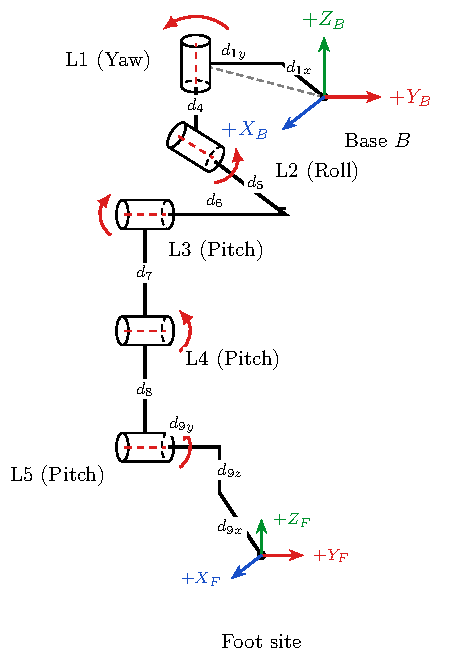
\includegraphics[width=95.040mm]{../assets/assignment_right_original.pdf}};
\draw[ink!50,densely dashed,line width=.5pt] (65.360,47.020)--(65.360,86.020);
\draw[ink!50,densely dashed,line width=.5pt] (55.280,63.420)--(98.280,95.920);
\draw[ink!50,densely dashed,line width=.5pt] (40.580,85.320)--(93.580,85.320);
\draw[ink!50,densely dashed,line width=.5pt] (40.580,109.740)--(74.580,109.740);
\draw[ink!50,densely dashed,line width=.5pt] (44.420,134.380)--(84.420,134.380);
\draw[al] (92.640,60.020)--(65.360,53.200);
\node[dimlabel,text=axa] at (79.000,50.610) {$a_0^{\rm DH}$};
\draw[dl] (65.360,53.200)--(65.360,71.020);
\node[dimlabel,text=axd] at (71.360,62.110) {$d_1^{\rm DH}$};
\draw[dl] (65.360,71.020)--(84.280,85.320);
\node[dimlabel,text=axd] at (78.820,73.170) {$d_2^{\rm DH}$};
\draw[dl] (84.280,85.320)--(54.580,85.320);
\draw[ink!65,line width=.4pt] (69.430,85.320)--(106.430,95.320);
\node[dimlabel,text=axd] at (106.430,95.320) {$d_3^{\rm DH}$};
\draw[al] (54.580,85.320)--(54.580,109.740);
\node[dimlabel,text=axa] at (47.580,97.530) {$a_3^{\rm DH}$};
\draw[al] (54.580,109.740)--(54.580,134.380);
\node[dimlabel,text=axa] at (47.580,122.060) {$a_4^{\rm DH}$};
\draw[dl] (54.580,134.380)--(70.420,134.380);
\node[dimlabel,text=axd] at (62.500,128.380) {$d_5^{\rm DH}$};
\draw[al] (70.420,134.380)--(79.220,140.980);
\node[dimlabel,text=axa] at (79.820,133.680) {$a_5^{\rm DH}$};
\draw[dl] (79.220,140.980)--(79.220,157.260);
\node[dimlabel,text=axd] at (96.220,149.120) {$d_6^{\rm DH}$};
\node[originmark] at (92.640,60.020) {};
\draw[ink!65,line width=.45pt] (92.640,60.020)--(108.640,37.020);
\node[fill=white,draw=ink!25,rounded corners=.6mm,inner sep=2pt,text=ink,font=\small] at (108.640,37.020) {\shortstack{$O_0=O_B$\\{\fontsize{7}{8}\selectfont \textcolor{axx}{$x_{0}=-sX-cY$}\;\textcolor{axy}{$y_{0}=cX-sY$}\;\textcolor{axz}{$z_{0}=+Z$}}}};
\node[originmark] at (65.360,53.200) {};
\draw[ink!65,line width=.45pt] (65.360,53.200)--(49.360,43.200);
\node[fill=white,inner sep=1pt,text=ink,font=\small] at (49.360,43.200) {$P_{1}$};
\node[originmark] at (65.360,71.020) {};
\draw[ink!65,line width=.45pt] (65.360,71.020)--(35.360,71.020);
\node[fill=white,draw=ink!25,rounded corners=.6mm,inner sep=2pt,text=ink,font=\small] at (35.360,71.020) {\shortstack{$O_{1}$\\{\fontsize{7}{8}\selectfont \textcolor{axx}{$x_{1}=+Y$}\;\textcolor{axy}{$y_{1}=-X$}\;\textcolor{axz}{$z_{1}=+Z$}}}};
\node[originmark] at (84.280,85.320) {};
\draw[ink!65,line width=.45pt] (84.280,85.320)--(111.280,81.320);
\node[fill=white,draw=ink!25,rounded corners=.6mm,inner sep=2pt,text=ink,font=\small] at (111.280,81.320) {\shortstack{$O_{2}$\\{\fontsize{7}{8}\selectfont \textcolor{axx}{$x_{2}=+Z$}\;\textcolor{axy}{$y_{2}=-Y$}\;\textcolor{axz}{$z_{2}=+X$}}}};
\node[originmark] at (54.580,85.320) {};
\draw[ink!65,line width=.45pt] (54.580,85.320)--(28.580,85.320);
\node[fill=white,draw=ink!25,rounded corners=.6mm,inner sep=2pt,text=ink,font=\small] at (28.580,85.320) {\shortstack{$O_{3}$\\{\fontsize{7}{8}\selectfont \textcolor{axx}{$x_{3}=-Z$}\;\textcolor{axy}{$y_{3}=-X$}\;\textcolor{axz}{$z_{3}=+Y$}}}};
\node[originmark] at (54.580,109.740) {};
\draw[ink!65,line width=.45pt] (54.580,109.740)--(28.580,109.740);
\node[fill=white,draw=ink!25,rounded corners=.6mm,inner sep=2pt,text=ink,font=\small] at (28.580,109.740) {\shortstack{$O_{4}$\\{\fontsize{7}{8}\selectfont \textcolor{axx}{$x_{4}=-Z$}\;\textcolor{axy}{$y_{4}=-X$}\;\textcolor{axz}{$z_{4}=+Y$}}}};
\node[originmark] at (54.580,134.380) {};
\draw[ink!65,line width=.45pt] (54.580,134.380)--(29.580,125.380);
\node[fill=white,inner sep=1pt,text=ink,font=\small] at (29.580,125.380) {$P_{5}$};
\node[originmark] at (70.420,134.380) {};
\draw[ink!65,line width=.45pt] (70.420,134.380)--(105.420,126.380);
\node[fill=white,draw=ink!25,rounded corners=.6mm,inner sep=2pt,text=ink,font=\small] at (105.420,126.380) {\shortstack{$O_{5}$\\{\fontsize{7}{8}\selectfont \textcolor{axx}{$x_{5}=+X$}\;\textcolor{axy}{$y_{5}=-Z$}\;\textcolor{axz}{$z_{5}=+Y$}}}};
\node[originmark] at (79.220,140.980) {};
\draw[ink!65,line width=.45pt] (79.220,140.980)--(95.220,137.980);
\node[fill=white,inner sep=1pt,text=ink,font=\small] at (95.220,137.980) {$P_{6}$};
\node[originmark] at (79.220,157.260) {};
\draw[ink!65,line width=.45pt] (79.220,157.260)--(104.220,168.260);
\node[fill=white,draw=ink!25,rounded corners=.6mm,inner sep=2pt,text=ink,font=\small] at (104.220,168.260) {\shortstack{$O_{6}$ (site)\\{\fontsize{7}{8}\selectfont \textcolor{axx}{$x_{6}=+X$}\;\textcolor{axy}{$y_{6}=+Y$}\;\textcolor{axz}{$z_{6}=+Z$}}}};
\node[anchor=north west,text=ink,font=\small] at (8.000,182.000) {\textcolor{axa}{Orange: $a_{i-1}^{\rm DH}$}\quad\textcolor{axd}{Purple: $d_i^{\rm DH}$}};
\node[anchor=north west,text=ink,text width=117mm,font=\footnotesize] at (8.000,190.000) {Original black $d$ labels are handout dimensions. Coloured superscript DH labels are table parameters.};
\node[anchor=north west,text=ink,font=\normalsize] at (137.000,34.000) {\textbf{Read each row as a two-step path}};
\node[anchor=north west,text=ink,font=\normalsize] at (137.000,43.000) {$O_{i-1}\xrightarrow[+x_{i-1}]{a_{i-1}}P_i\xrightarrow[+z_i]{d_i}O_i$};
\node[anchor=north west,text=ink,font=\small] at (137.000,54.000) {A negative value means travel opposite to that positive axis.};
\node[anchor=north west,text=ink,font=\small,inner sep=0pt] at (138.000,63.000) {\begin{tabular}{c|rr|cc}
$i$ & $a_{i-1}$ & $d_i$ & axis for $a$ & axis for $d$\\\hline
$1$ & $39.8246$ & $-0.0741$ & $-sX-cY$ & $+Z$\\
$2$ & $0$ & $-16.06$ & $+Y$ & $+X$\\
$3$ & $0$ & $-74.15$ & $+Z$ & $+Y$\\
$4$ & $78.65$ & $0$ & $-Z$ & $+Y$\\
$5$ & $78.65$ & $17.35$ & $-Z$ & $+Y$\\
$6$ & $0.5$ & $-36.225$ & $+X$ & $+Z$\\
\end{tabular}};
\node[anchor=north west,text=ink,font=\footnotesize,align=left] at (137.000,102.000) {$a_1=a_2=0$; $d_4=0$.\\$P_2=O_1$, $P_3=O_2$, $P_4=O_4$.};
\node[anchor=north west,text=ink,font=\normalsize] at (137.000,114.000) {\textbf{Full frame axes, expressed in base $B$}};
\node[anchor=north west,text=ink,font=\small,inner sep=0pt] at (138.000,124.000) {\begin{tabular}{c|ccc}
frame & \textcolor{axx}{$+x_i$} & \textcolor{axy}{$+y_i$} & \textcolor{axz}{$+z_i$}\\\hline
$0$ & $-sX-cY$ & $cX-sY$ & $+Z$\\
$1$ & $+Y$ & $-X$ & $+Z$\\
$2$ & $+Z$ & $-Y$ & $+X$\\
$3$ & $-Z$ & $-X$ & $+Y$\\
$4$ & $-Z$ & $-X$ & $+Y$\\
$5$ & $+X$ & $-Z$ & $+Y$\\
$6$ & $+X$ & $+Y$ & $+Z$\\
\end{tabular}};
\node[anchor=north west,text=ink,font=\footnotesize,text width=56mm,align=center] at (231.000,61.000) {\textbf{Positive-axis triads}\newline Translated from their $O_i$};
\node[text=ink,font=\small] at (244.000,75.000) {$i=0$};
\draw[-{Latex[length=1.4mm]},axx,line width=.8pt] (244.000,87.000)--(238.359,84.956);
\node[text=axx,font=\footnotesize,inner sep=0pt] at (235.914,85.071) {$x_i$};
\draw[-{Latex[length=1.4mm]},axy,line width=.8pt] (244.000,87.000)--(238.417,89.198);
\node[text=axy,font=\footnotesize,inner sep=0pt] at (235.998,90.151) {$y_i$};
\draw[-{Latex[length=1.4mm]},axz,line width=.8pt] (244.000,87.000)--(244.000,81.000);
\node[text=axz,font=\footnotesize,inner sep=0pt] at (244.000,78.400) {$z_i$};
\fill[ink] (244.000,87.000) circle[radius=.45mm];
\node[text=ink,font=\small] at (274.000,75.000) {$i=1$};
\draw[-{Latex[length=1.4mm]},axx,line width=.8pt] (274.000,87.000)--(280.000,87.000);
\node[text=axx,font=\footnotesize,inner sep=0pt] at (282.600,87.000) {$x_i$};
\draw[-{Latex[length=1.4mm]},axy,line width=.8pt] (274.000,87.000)--(278.800,83.400);
\node[text=axy,font=\footnotesize,inner sep=0pt] at (280.880,81.840) {$y_i$};
\draw[-{Latex[length=1.4mm]},axz,line width=.8pt] (274.000,87.000)--(274.000,81.000);
\node[text=axz,font=\footnotesize,inner sep=0pt] at (274.000,78.400) {$z_i$};
\fill[ink] (274.000,87.000) circle[radius=.45mm];
\node[text=ink,font=\small] at (244.000,104.000) {$i=2$};
\draw[-{Latex[length=1.4mm]},axx,line width=.8pt] (244.000,116.000)--(244.000,110.000);
\node[text=axx,font=\footnotesize,inner sep=0pt] at (244.000,107.400) {$x_i$};
\draw[-{Latex[length=1.4mm]},axy,line width=.8pt] (244.000,116.000)--(238.000,116.000);
\node[text=axy,font=\footnotesize,inner sep=0pt] at (235.400,116.000) {$y_i$};
\draw[-{Latex[length=1.4mm]},axz,line width=.8pt] (244.000,116.000)--(239.200,119.600);
\node[text=axz,font=\footnotesize,inner sep=0pt] at (237.120,121.160) {$z_i$};
\fill[ink] (244.000,116.000) circle[radius=.45mm];
\node[text=ink,font=\small] at (274.000,104.000) {$i=3,4$};
\draw[-{Latex[length=1.4mm]},axx,line width=.8pt] (274.000,116.000)--(274.000,122.000);
\node[text=axx,font=\footnotesize,inner sep=0pt] at (274.000,124.600) {$x_i$};
\draw[-{Latex[length=1.4mm]},axy,line width=.8pt] (274.000,116.000)--(278.800,112.400);
\node[text=axy,font=\footnotesize,inner sep=0pt] at (280.880,110.840) {$y_i$};
\draw[-{Latex[length=1.4mm]},axz,line width=.8pt] (274.000,116.000)--(280.000,116.000);
\node[text=axz,font=\footnotesize,inner sep=0pt] at (282.600,116.000) {$z_i$};
\fill[ink] (274.000,116.000) circle[radius=.45mm];
\node[text=ink,font=\small] at (244.000,133.000) {$i=5$};
\draw[-{Latex[length=1.4mm]},axx,line width=.8pt] (244.000,145.000)--(239.200,148.600);
\node[text=axx,font=\footnotesize,inner sep=0pt] at (237.120,150.160) {$x_i$};
\draw[-{Latex[length=1.4mm]},axy,line width=.8pt] (244.000,145.000)--(244.000,151.000);
\node[text=axy,font=\footnotesize,inner sep=0pt] at (244.000,153.600) {$y_i$};
\draw[-{Latex[length=1.4mm]},axz,line width=.8pt] (244.000,145.000)--(250.000,145.000);
\node[text=axz,font=\footnotesize,inner sep=0pt] at (252.600,145.000) {$z_i$};
\fill[ink] (244.000,145.000) circle[radius=.45mm];
\node[text=ink,font=\small] at (274.000,133.000) {$i=6$};
\draw[-{Latex[length=1.4mm]},axx,line width=.8pt] (274.000,145.000)--(269.200,148.600);
\node[text=axx,font=\footnotesize,inner sep=0pt] at (267.120,150.160) {$x_i$};
\draw[-{Latex[length=1.4mm]},axy,line width=.8pt] (274.000,145.000)--(280.000,145.000);
\node[text=axy,font=\footnotesize,inner sep=0pt] at (282.600,145.000) {$y_i$};
\draw[-{Latex[length=1.4mm]},axz,line width=.8pt] (274.000,145.000)--(274.000,139.000);
\node[text=axz,font=\footnotesize,inner sep=0pt] at (274.000,136.400) {$z_i$};
\fill[ink] (274.000,145.000) circle[radius=.45mm];
\node[anchor=north west,text=ink,font=\footnotesize] at (138.000,160.000) {$s=\sin\beta$, $c=\cos\beta$, $\beta=\operatorname{atan2}(19,35)$.};
\node[anchor=north west,text=ink,text width=149mm,font=\footnotesize,align=left] at (137.000,166.000) {$O_1$: yaw/roll axis intersection. $O_2$: roll/hip-pitch axis intersection. $P_5$ and $O_5$ share the ankle axis. $P_6$ is the auxiliary corner for the D-H translation order. $O_0=B$. The first vertical segment ends at $O_1$; $d_1=-0.0741$ mm. Cylinder centres are not assumed to be D-H origins.};
\node[anchor=north west,text=ink,text width=149mm,font=\footnotesize,align=left] at (137.000,192.000) {Original: Assignment 1, Fig. 3. Schematic, not to scale; perspective is illustrative. Exact signs and directions are given in the tables. Markers are selected D-H origins, not CAD joint centres.};
\end{scope}
\end{tikzpicture}
\end{document}
